%%%%%%%%%%%%%%%%%%%%%%%%%%%%%%%%%
%% PROPOSITO GENERAL
%%%%%%%%%%%%%%%%%%%%%%%%%%%%%%%%%
\subsubsection{Propósito}

Docker es una plataforma abierta que tiene como propósito permitir el desarrollo, envío y ejecución de aplicaciones, permitiendo separar el software de la infraestructura para que se pueda entregar software rápidamente \parencite{Docker2018}.

Es importante aclarar que Docker tiene tanto una versión empresarial llamada Docker EE (Enterprise Edition) y una versión comunitaria llamada Docker CE (Community Edition) ver figura \ref{fig:DockerVersiones}. Para el presente trabajo se utiliza la versión comunitaria.

\begin{figure}[!hbtp]
	\centering
	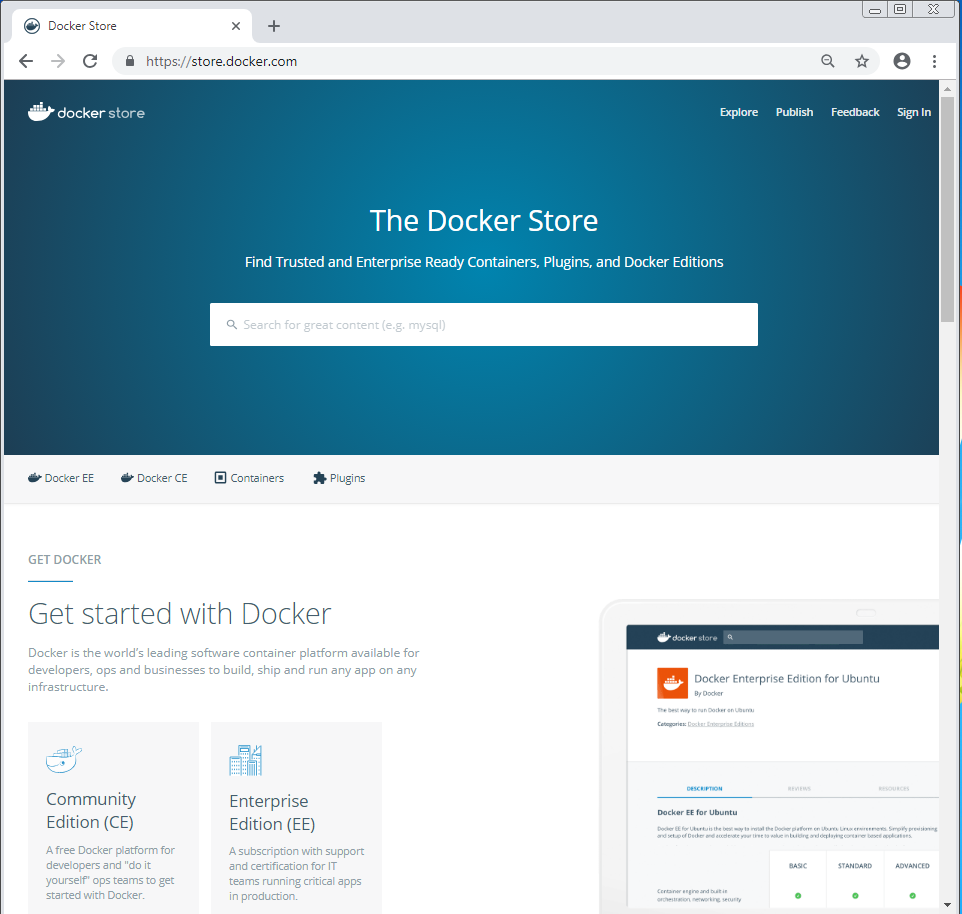
\includegraphics[width=\linewidth]{Trabajo/RecursosEducativos/RE05_Docker/REDocker_versiones.png}
	\vspace{-0.2cm}
	\caption{Sitio web The Docker Store \url{https://store.docker.com/}. }
	\label{fig:DockerVersiones}
\end{figure}

%%%%%%%%%%%%%%%%%%%%%%%%%%%%%%%%%
%% ASPECTOS TEC GENERALES
%%%%%%%%%%%%%%%%%%%%%%%%%%%%%%%%%

\subsection{Aspectos técnicos generales}

Según \textcite{Docker2018} Docker ofrece la capacidad de empaquetar y ejecutar aplicaciones en un entorno aislado y holgado llamado contenedor, el aislamiento y la seguridad permite ejecutar muchos contenedores simultáneamente en un mismo host. Adicional \textcite{Docker2018} indica que los contenedores son livianos porque no necesitan la carga de un hipervisor, debido a que se ejecutan directamente en el nucleo del equipo host, incluso dentro de máquinas virtuales que se encuentren en un host.

Docker proporciona una plataforma y herramientas para la administración del ciclo de vida de sus contenedores:
\begin{itemize}
    \item Desarrolle sus aplicaciones y componentes de soporte utilizando Docker.
    \item El contenedor creado se convierte en la unidad para distribuir y probar la aplicación.
    \item Cuanto todo este listo y funcional, puede desplegar la aplicación o el servicio en producción de la misma forma sin importar que el entorno de producción sea un datacenter, una nube pública o privada.
\end{itemize}

Según \textcite{Docker2018} cuando se utiliza Docker se crean y se utilizan contenedores, imágenes, volúmenes, redes, complementos, entre otras cosas. En esta sección se procede a describir que es una imagen y un contenedor.

\textbf{Imágenes}
Una imagen es una plantilla de solo lectura con instrucciones para crear un contenedor Docker. A menudo, una imagen se basa en otra imagen, con alguna personalización adicional. Por ejemplo, puede crear una imagen basada en la imagen de ubuntu, pero instala el servidor web Apache y su aplicación, así como los detalles de configuración necesarios para hacer que su aplicación se ejecute. \parencite{Docker2018}.

\textbf{Contenedores}
Un contenedor es una instancia ejecutable de una imagen. Puede crear, iniciar, detener, mover o eliminar un contenedor utilizando la API o la CLI de Docker. Puede conectar un contenedor a una o más redes, adjuntarle almacenamiento o incluso crear una nueva imagen según su estado actual. Un contenedor se define por su imagen, así como por las opciones de configuración que le proporciona al crearlo o iniciarlo. Cuando se elimina un contenedor, desaparecen todos los cambios en su estado que no se almacenan en el almacenamiento persistente. \parencite{Docker2018}


%%%%%%%%%%%%%%%%%%%%%%%%%%%%%%%%%
%% ARQUITECTURA
%%%%%%%%%%%%%%%%%%%%%%%%%%%%%%%%%
\subsubsection{Arquitectura}

Como se puede observar en la figura \ref{fig:DockerArquitectura} y según lo establece \textcite{Docker2018} Docker utiliza una arquitectura de cliente servidor. En la cual el cliente Docker habla con el Demonio de Docker encargado de construir, ejecutar y distribuir los contenedores Docker. El cliente y el demonio pueden estar en ejecución en el mismo host o en host remotos, debido a que se pueden comunicar a través de API Rest, Sockets Unix o interfaces de red.

\begin{figure}[!hbtp]
	\centering
	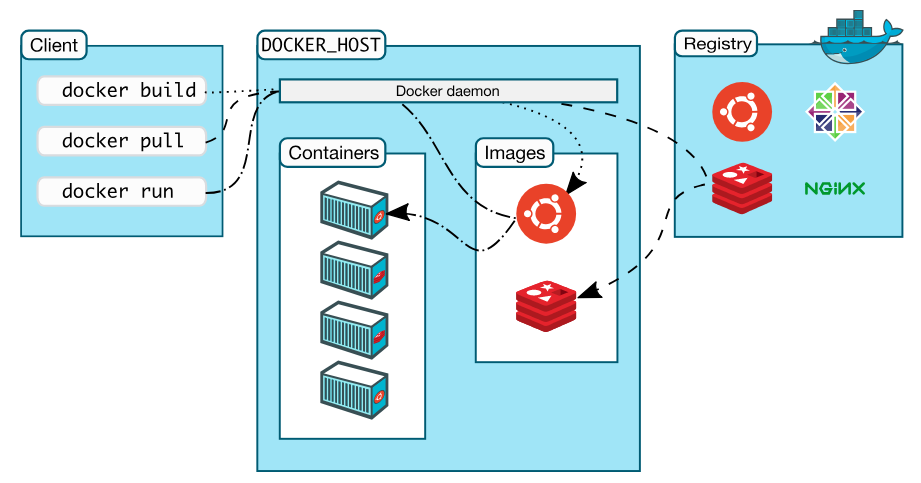
\includegraphics[width=\linewidth]{Trabajo/RecursosEducativos/RE05_Docker/REDocker_Arquitectura.png}
	\vspace{-0.2cm}
	\caption{Sitio web Docker Docs \url{https://docs.docker.com/engine/docker-overview/}.}
	\label{fig:DockerArquitectura}
\end{figure}

En la figura \ref{fig:DockerArquitectura} se encuentran los siguientes componentes:
\textbf{The Docker Daemon (El demonio de docker)}
El demonio de Docker (dockerd) escucha las solicitudes de la API de Docker y administra los objetos de Docker, como imágenes, contenedores, redes y volúmenes. Un demonio también puede comunicarse con otros demonios para administrar los servicios de Docker. \parencite{Docker2018}

\textbf{The Docker Client (El cliente de Docker)}
El cliente Docker (docker) es la forma principal en que muchos usuarios de Docker interactúan con Docker. Cuando utiliza comandos como la ejecución de la ventana acoplable, el cliente envía estos comandos a dockerd, que los ejecuta. El comando docker utiliza la API de Docker. El cliente Docker puede comunicarse con más de un demonio.\parencite{Docker2018}

\textbf{Docker Registries (Registros de Docker)}
Un registro de Docker es donde se almacenan las imágenes de Docker. Docker Hub es un registro público que cualquiera puede usar. Docker está configurado para buscar imágenes en Docker Hub de forma predeterminada. Es posible tener un registro de imágenes privado. \parencite{Docker2018}

%%%%%%%%%%%%%%%%%%%%%%%%%%%%%%%%%
%% INSTALACION LINUX
%%%%%%%%%%%%%%%%%%%%%%%%%%%%%%%%%
\subsection{Instalación en Linux}
Para la instalación de Docker CE en los sistemas operativos GNU/Linux se tienen diferentes métodos como la instalación de los repositorios, descargar los ejecutables para la distribución específica o la ejecución de un script que contiene los pasos de instalación básica, la ejecución del script se realiza con los siguientes comandos, y su salida se puede observar en la figura \ref{fig:InstalacionDockerLinux1}

\begin{figure}[!hbtp]
	\centering
	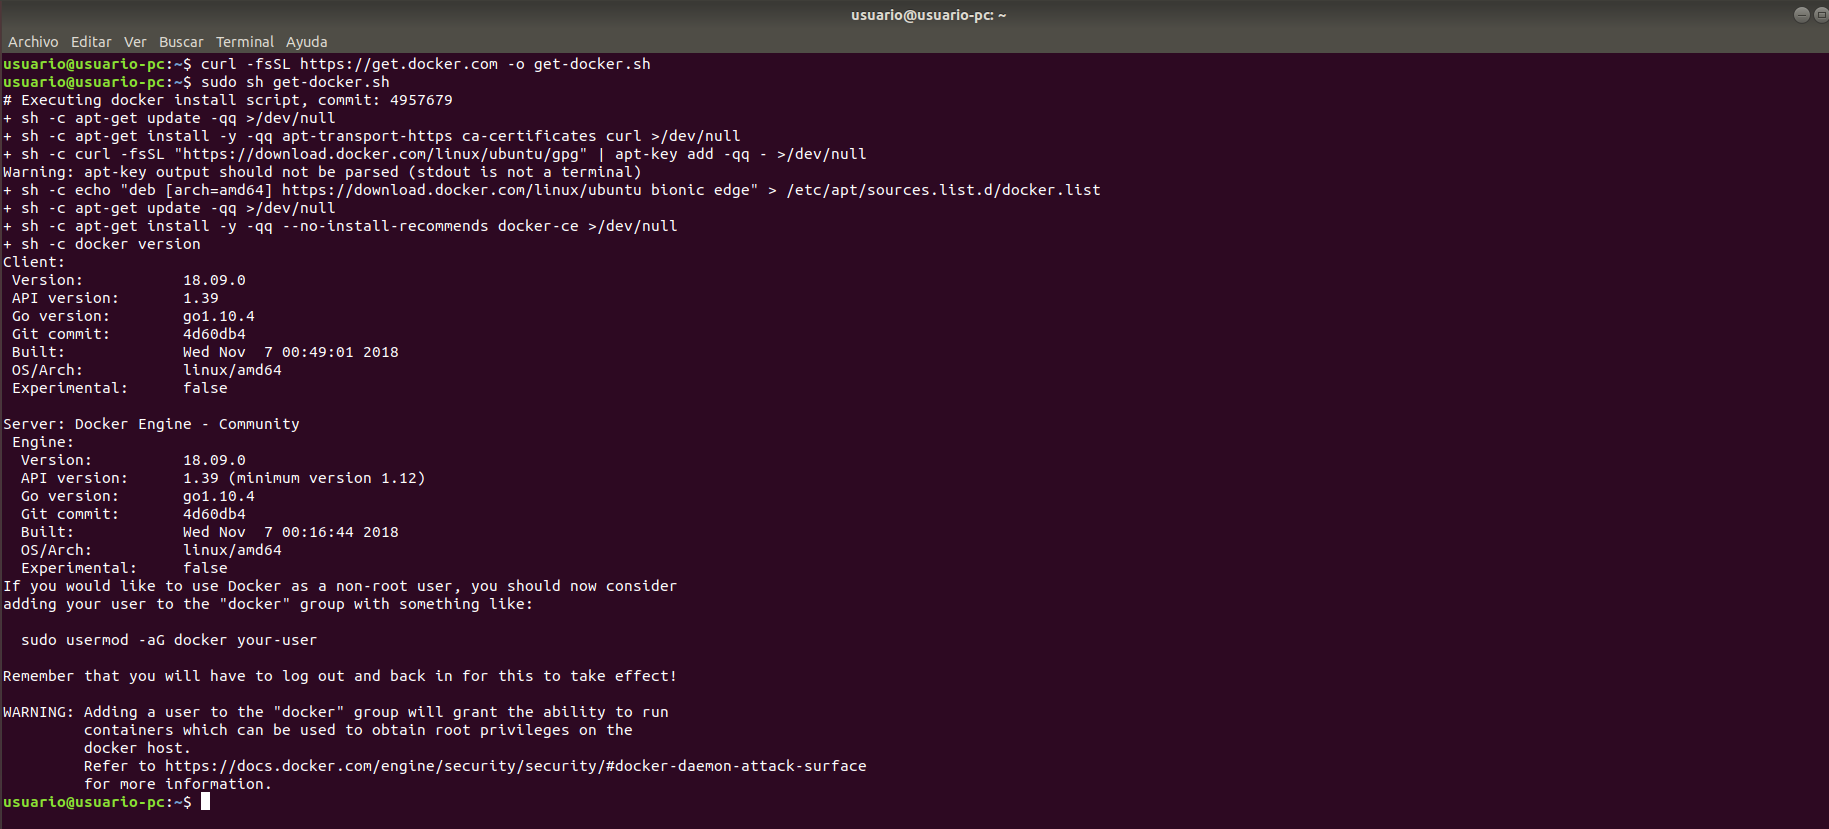
\includegraphics[width=\linewidth]{Trabajo/RecursosEducativos/RE05_Docker/Instalacion_Linux/REDocker_Instalacion_Linux.png}
	\vspace{-0.2cm}
	\caption{Salida del script de instalación Docker }
	\label{fig:InstalacionDockerLinux1}
\end{figure}

Al terminar la instalación de Docker CE se puede verificar la versión básica de Docker con el comando \begin{commandshell}{docker version}\end{commandshell}
en la figura \ref{fig:InstalacionDockerLinux2} se puede ver la salida del comando.

\begin{figure}[!hbtp]
	\centering
	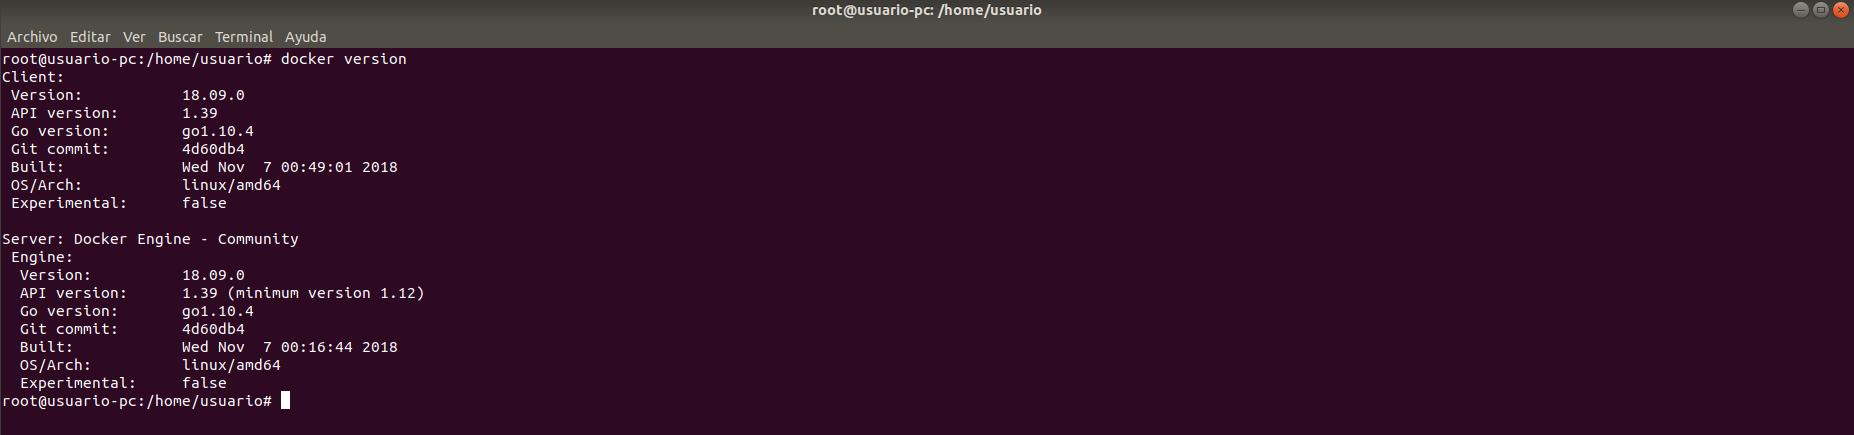
\includegraphics[width=\linewidth]{Trabajo/RecursosEducativos/RE05_Docker/Instalacion_Linux/REDocker_Instalacion_Linux2.png}
	\vspace{-0.2cm}
	\caption{Salida del comando docker version }
	\label{fig:InstalacionDockerLinux2}
\end{figure}
%%%%%%%%%%%%%%%%%%%%%%%%%%%%%%%%%
%% INSTALACION Windows
%%%%%%%%%%%%%%%%%%%%%%%%%%%%%%%%%
\subsection{Instalación Microsoft Windows}
Para poder realizar la instalación de Docker en microsoft windows de una forma nativa, sólo funcionará con las versiones Microsoft Windows 10 Professional y Microsoft Windows 10 Enterprise, en las figuras \ref{fig:InstalacionDockerWin1},\ref{fig:InstalacionDockerWin2},\ref{fig:InstalacionDockerWin3},\ref{fig:InstalacionDockerWin4} se muestra la interacción con el asistente de instalación de Docker.

\begin{figure}[!hbtp]
	\centering
	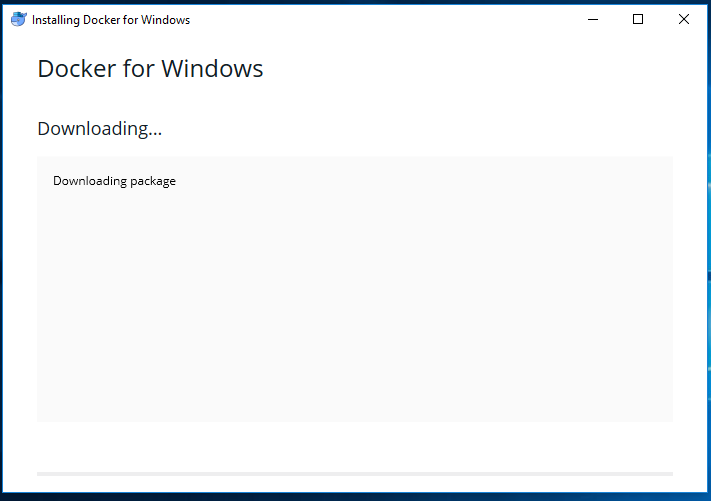
\includegraphics[width=\linewidth]{Trabajo/RecursosEducativos/RE05_Docker/Instalacion_Windows/REDocker_Instalacion_Windows01.png}
	\vspace{-0.2cm}
	\caption{Asistente instalación Docker: Descarga paquetes necesarios}
	\label{fig:InstalacionDockerWin1}
\end{figure}

\begin{figure}[!hbtp]
	\centering
	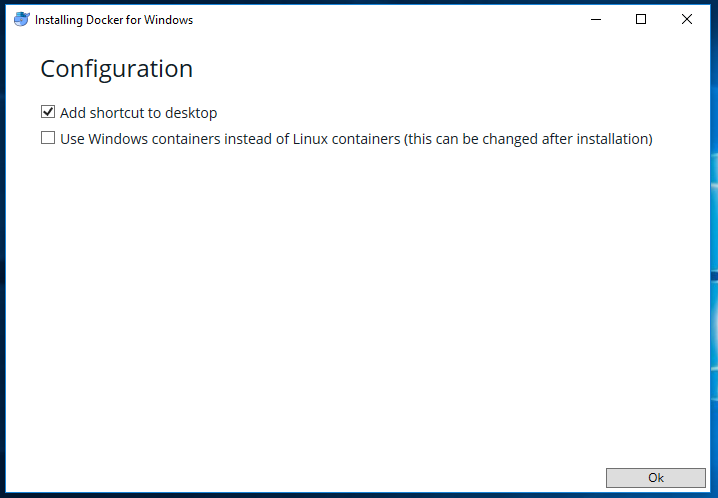
\includegraphics[width=\linewidth]{Trabajo/RecursosEducativos/RE05_Docker/Instalacion_Windows/REDocker_Instalacion_Windows02.png}
	\vspace{-0.2cm}
	\caption{Asistente instalación Docker: Configuración básica}
	\label{fig:InstalacionDockerWin2}
\end{figure}

\begin{figure}[!hbtp]
	\centering
	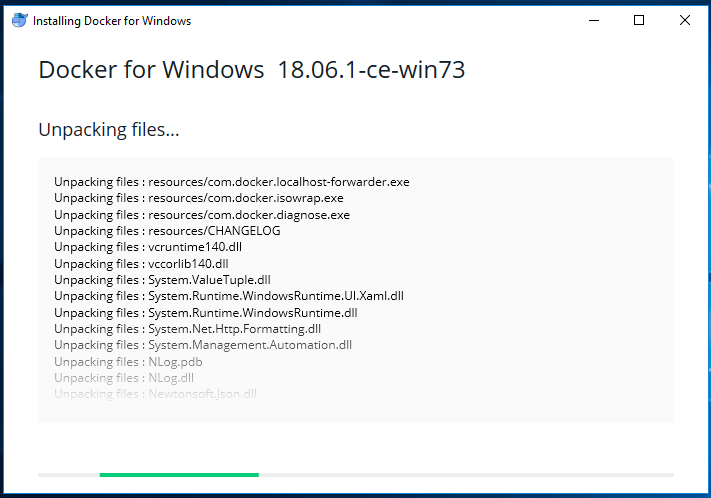
\includegraphics[width=\linewidth]{Trabajo/RecursosEducativos/RE05_Docker/Instalacion_Windows/REDocker_Instalacion_Windows03.png}
	\vspace{-0.2cm}
	\caption{Asistente instalación Docker: Descompresión de paquetes}
	\label{fig:InstalacionDockerWin3}
\end{figure}

\begin{figure}[!hbtp]
	\centering
	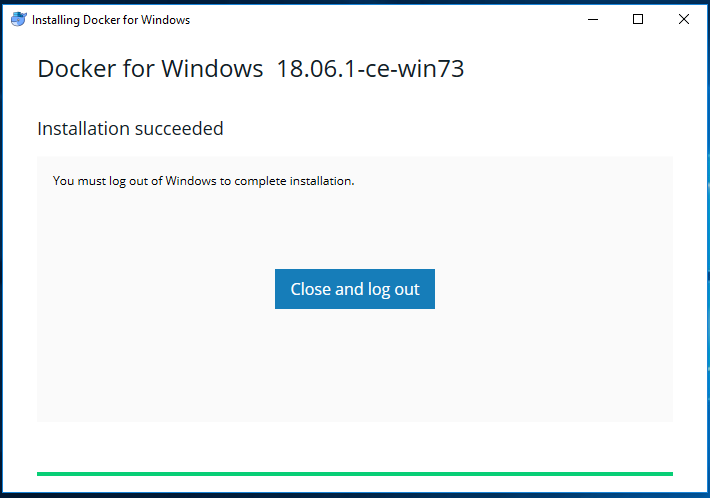
\includegraphics[width=\linewidth]{Trabajo/RecursosEducativos/RE05_Docker/Instalacion_Windows/REDocker_Instalacion_Windows04.png}
	\vspace{-0.2cm}
	\caption{Asistente instalación Docker: Finalización del asistente}
	\label{fig:InstalacionDockerWin4}
\end{figure}

En caso de que se tengan versiones de Microsoft Windows anteriores se puede utilizar Docker Tool Box, herramienta que permite a través de una máquina virtual la gestión de contenedores Docker. Para conocer el proceso de instalación se puede ver el Anexo 2.

%%%%%%%%%%%%%%%%%%%%%%%%%%%%%%%%%
%% GESTION BÁSICA 
%%%%%%%%%%%%%%%%%%%%%%%%%%%%%%%%%
\subsection{Gestión básica de Docker}

Es esta sección s van a mostrar algunos comandos básicos para la gestión básica de imagenes, contenedores, entre otros.

\textbf{Consulta de información Docker}

Para ver la información general de la instalación de docker sus contenedores, imagenes y demás información relevante se utiliza el comando \begin{commandshell}docker info\end{commandshell} 
en la figura \ref{fig:DockerGestion1} se puede ver la salida del comando.

\begin{figure}[!hbtp]
	\centering
	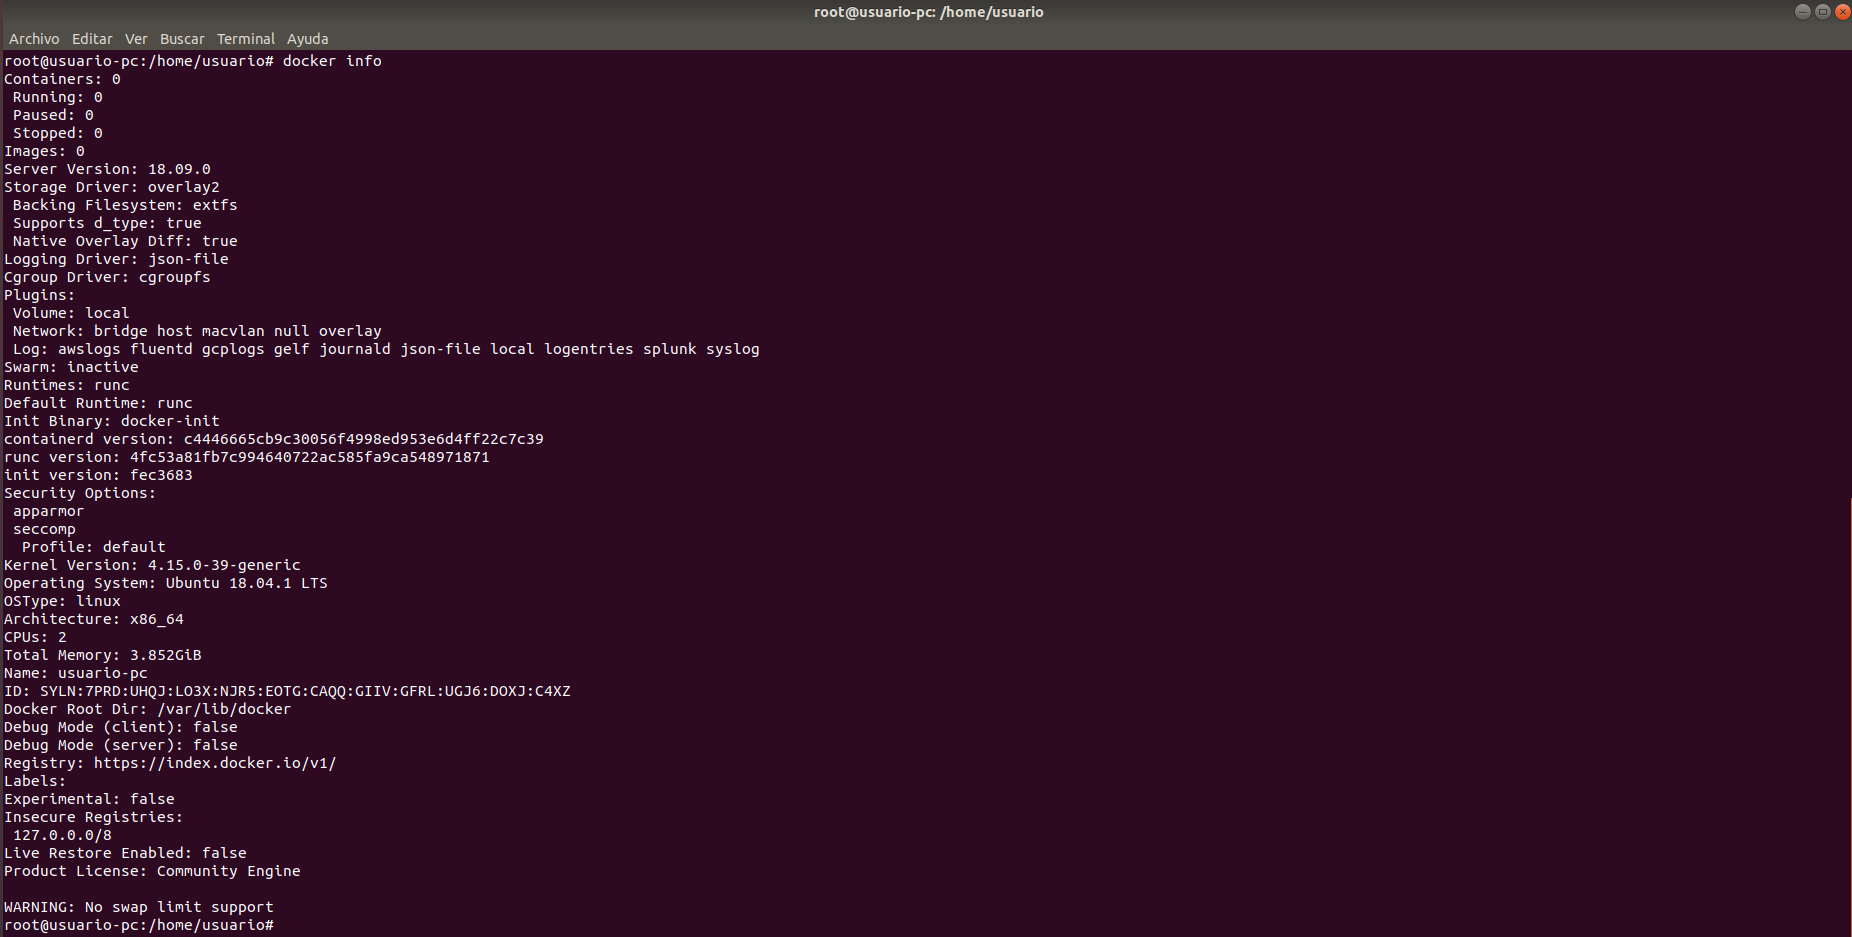
\includegraphics[width=\linewidth]{Trabajo/RecursosEducativos/RE05_Docker/Gestion_basica/REDocker_Gestion1.png}
	\vspace{-0.2cm}
	\caption{Salida del comando docker info}
	\label{fig:DockerGestion1}
\end{figure}
%%%%%%%%%%%%%%%%%%%%%%%%%%%%%%%%%
%% GESTIÓN DE IMAGENES
%%%%%%%%%%%%%%%%%%%%%%%%%%%%%%%%%
\textbf{Consulta de imágenes existentes en el host}

Para listar las imágenes descargadas en el host que actualmente ejecuta docker se utiliza el siguiente comando  \begin{commandshell}docker images\end{commandshell}

En la imagen \ref{fig:DockerGestion2} se puede observar la salida del comando destacando la siguiente información:
\begin{itemize}
    \item REPOSITORY: Nombre del repositorio donde proviene la imagen.
    \item TAG: Es utilizado para nombrar las versiones de una imagen, es decir, a medida que se se introducen cambios a una imagen se puede asociar con un nuevo TAG, facilitando el control de versiones de las imagenes.
    \item IMAGE ID: Número de identificación único para cada imagen.
    \item CREATE: Indica el momento en el que fue creada la imagen.
    \item SIZE: Indica el tamaño en disco de la imagen.
\end{itemize}

\begin{figure}[!hbtp]
	\centering
	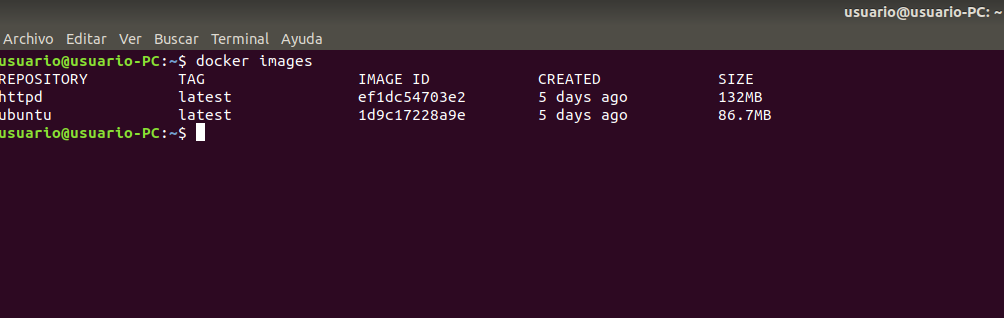
\includegraphics[width=\linewidth]{Trabajo/RecursosEducativos/RE05_Docker/Gestion_basica/REDocker_Gestion2.png}
	\vspace{-0.2cm}
	\caption{Salida del comando docker images}
	\label{fig:DockerGestion2}
\end{figure}
%%%%%%%%%%%%%%%%%%%%%%%%%%%%%%%%%
%% BUSQUEDA EN DOCKER HUB
%%%%%%%%%%%%%%%%%%%%%%%%%%%%%%%%%
\textbf{Búsqueda de imágenes en repositorio}

Docker apoyado en su comunidad a través de Docker Hub ver figura \ref{fig:DockerGestion4} ofrece un servicio para buscar y compartir imágenes de contenedores. Para poder buscar las imagenes disponibles es necesaria la creación de una cuenta.

\begin{figure}[!hbtp]
	\centering
	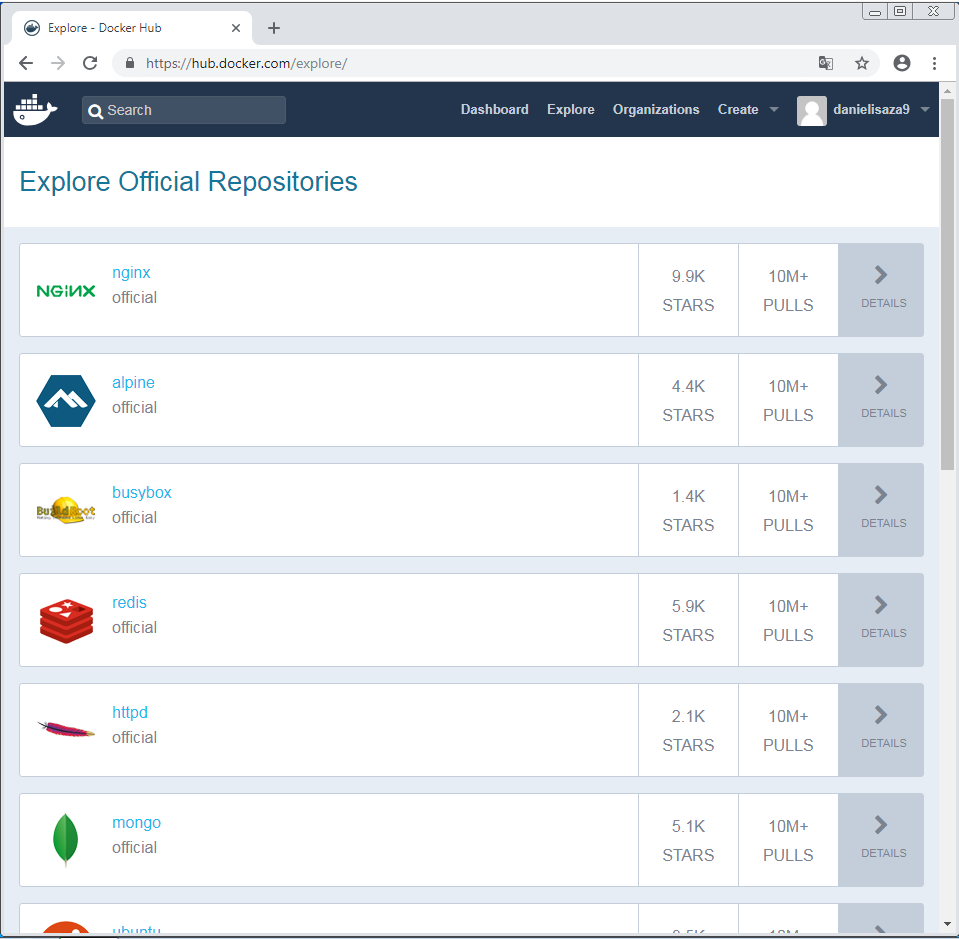
\includegraphics[width=\linewidth]{Trabajo/RecursosEducativos/RE05_Docker/Gestion_basica/REDocker_Gestion4.png}
	\vspace{-0.2cm}
	\caption{Sitio web Docker Hub \url{https://hub.docker.com/explore/}.}
	\label{fig:DockerGestion4}
\end{figure}

Para buscar una imagen alojada en Docker Hub para su posible descarga se utiliza el comando 
\begin{commandshell}docker search nombreImagen\end{commandshell}

En la figura \ref{fig:DockerGestion3} se ve la salida del comando para la búsqueda de imágenes que tengan la palabra ubuntu.

\begin{figure}[!hbtp]
	\centering
	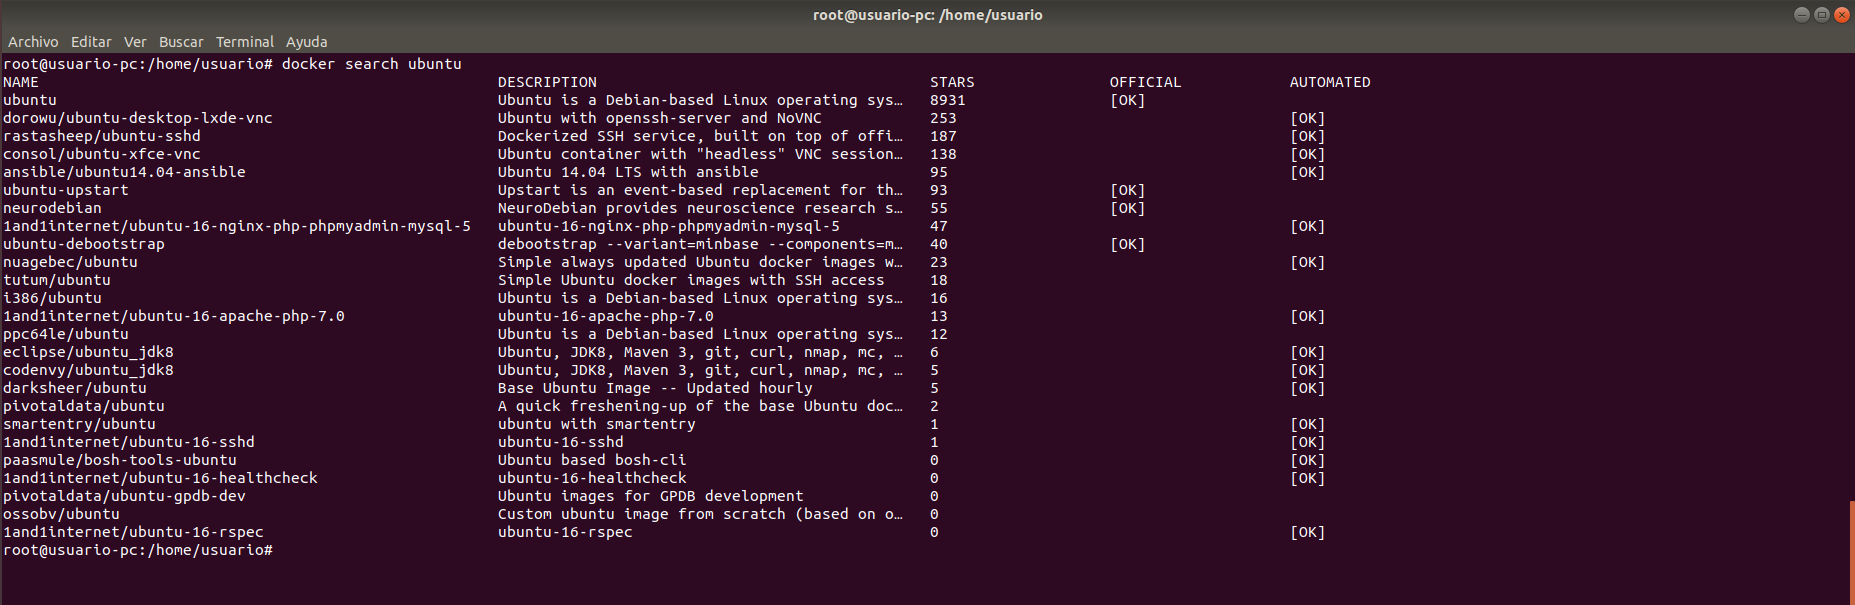
\includegraphics[width=\linewidth]{Trabajo/RecursosEducativos/RE05_Docker/Gestion_basica/REDocker_Gestion3.png}
	\vspace{-0.2cm}
	\caption{Salida comando docker search ubuntu}
	\label{fig:DockerGestion3}
\end{figure}

%%%%%%%%%%%%%%%%%%%%%%%%%%%%%%%%%
%% DESCARGA IMAGENES
%%%%%%%%%%%%%%%%%%%%%%%%%%%%%%%%%
\textbf{Descarga de una imagen}
Una vez que se identifica el nombre de la imagen que se desea descargar de Docker Hub, por ejemplo la imagen hello-world que se envia como argumento del comando pull de la siguiente forma:
\begin{commandshell} docker pull hello-world \end{commandshell}

La salida del comando se puede observar en la figura \ref{fig:DockerGestion5} donde se muestra la descarga exitosa de la imagen y la verificación de que la misma exista. 

\begin{figure}[!hbtp]
	\centering
	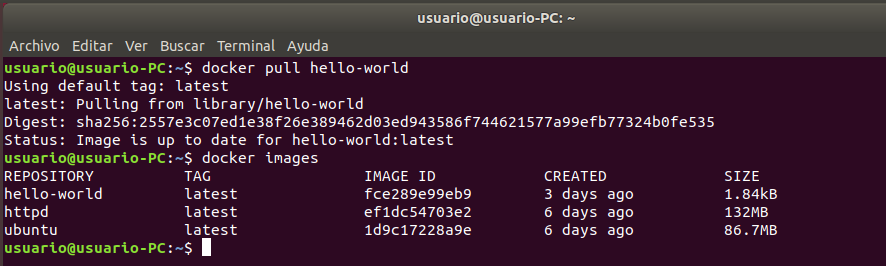
\includegraphics[width=\linewidth]{Trabajo/RecursosEducativos/RE05_Docker/Gestion_basica/REDocker_Gestion5.png}
	\vspace{-0.2cm}
	\caption{Salida comando docker search ubuntu}
	\label{fig:DockerGestion5}
\end{figure}

También es posible agregar el TAG al comando de descarga de imágenes, permitiendo establecer la versión especifica que se desea obtener, como se muestra en el siguiente comando:

\begin{commandshell} docker pull hello-world:latest \end{commandshell}

%%%%%%%%%%%%%%%%%%%%%%%%%%%%%%%%%
%% CREACION CONTENEDORES
%%%%%%%%%%%%%%%%%%%%%%%%%%%%%%%%%
\textbf{Creación de un contenedor}
Para poder crear un nuevo contenedor es necesario conocer el nombre de la imagen que se desea utilizar, no es necesario que la imagen se encuentre disponible localmente, en dicho caso docker procede con la búsqueda y descarga desde Docker Hub.  

Un ejemplo de imagen clásico es la de hello-world que sigue la tradición del primer programa que se crea cuando se aprende a programar, el comando para crear el contenedor es el siguiente

\begin{commandshell} docker run hello-world \end{commandshell}

En la figura \ref{fig:DockerGestion6} se puede observar la salida del comando y se puede identificar que al ejecutar un contenedor utilizando la imagen hello-world se verifica el correcto funcionamiento de docker.

\begin{figure}[!hbtp]
	\centering
	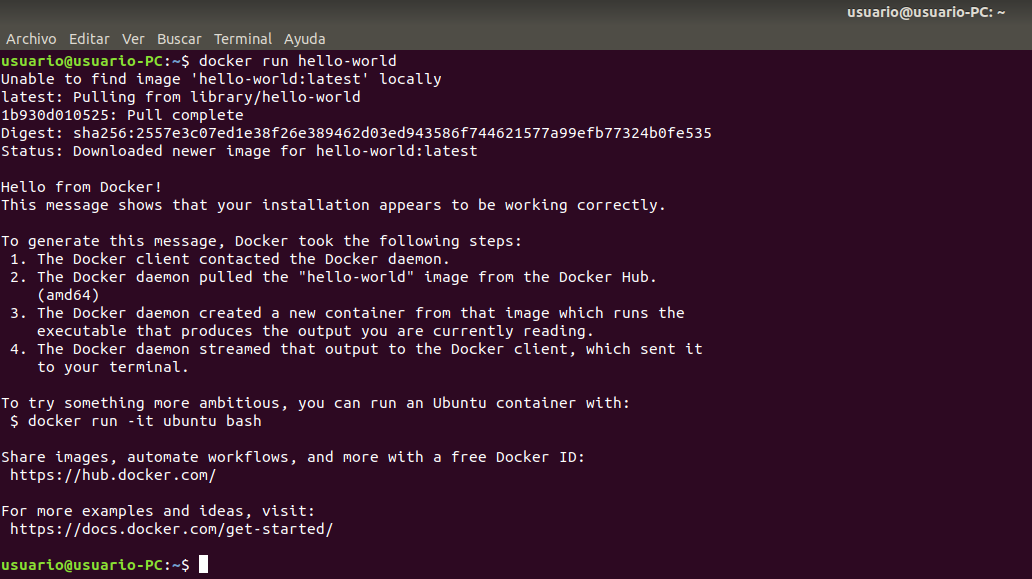
\includegraphics[width=\linewidth]{Trabajo/RecursosEducativos/RE05_Docker/Gestion_basica/REDocker_Gestion6.png}
	\vspace{-0.2cm}
	\caption{Salida comando docker run hello-world}
	\label{fig:DockerGestion6}
\end{figure}

Para listar los contenedores que se han creado en el host ya sea que se encuentren en ejecución se utiliza el siguiente comando
\begin{commandshell} docker ps \end{commandshell}

En caso de que se deseen ver todos los contenedores en ejecución y que ya se encuentran detenidos, se agrega la opción -a tal como se ve en el siguiente comando
\begin{commandshell} docker ps -a \end{commandshell}

La salida de los comandos mostrados anteriormente se ve reflejada en la figura \ref{fig:DockerGestion7}, la cual contiene la siguiente información: 
\begin{itemize}
    \item CONTAINER ID: Número único de identificación para el contenedor en el host actual.
    \item IMAGE: Nombre de la imagen y etiqueta utilizados para la creación del contenedor.
    \item COMMAND: Hace referencia al comando citado al momento de ejecutar el contenedor.
    \item CREATED: Indica el momento de creación del contenedor.
    \item STATUS: Muestra el estado del contenedor, en caso de que se encuentre detenido indica el tiempo de terminación.
    \item PORTS: Indica el puerto TCP del host que se utiliza para escuchar un puerto específico del contenedor.
    \item NAMES: Hace referencia al nombre dado al contenedor ya sea de forma aleatoria o manual. 
\end{itemize}

\begin{figure}[!hbtp]
	\centering
	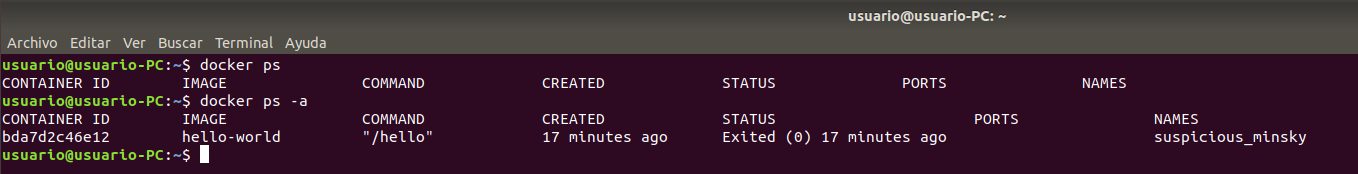
\includegraphics[width=\linewidth]{Trabajo/RecursosEducativos/RE05_Docker/Gestion_basica/REDocker_Gestion7.png}
	\vspace{-0.2cm}
	\caption{Salida comandos docker ps  docker ps -a}
	\label{fig:DockerGestion7}
\end{figure}
%%%%%%%%%%%%%%%%%%%%%%%%%%%%%%%%%
%% EJECUCION COMANDOS CONTENEDORES
%%%%%%%%%%%%%%%%%%%%%%%%%%%%%%%%%
\textbf{Ejecutar comandos en contenedores}
A través del comando \texttt{docker run} es posible crear contenedores y ejecutar comandos en los mismos. Por ejemplo, para ejecutar el comando ls -l en un contenedor creado con una imagen de ubuntu, se deben ejecutar los siguientes comandos:
\begin{commandshell}
docker pull ubuntu:latest
docker run ubuntu ls -l /
\end{commandshell}

El resultado de la ejecución del comando ls -l en ubuntu, se puede observar en la figura \ref{fig:DockerGestion8} donde se ven los directorios ubicados en raíz.

\begin{figure}[!hbtp]
	\centering
	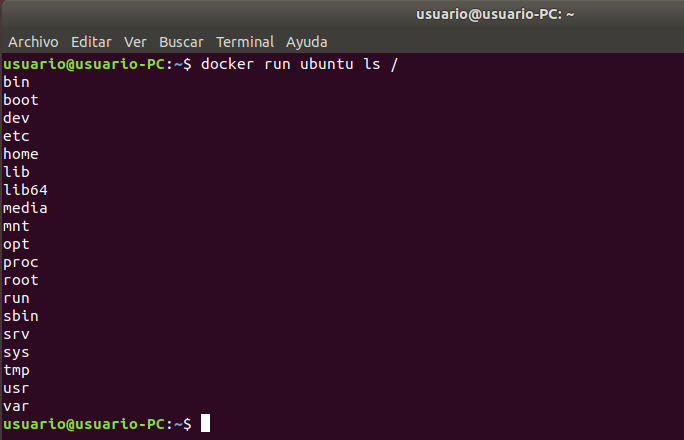
\includegraphics[width=\linewidth]{Trabajo/RecursosEducativos/RE05_Docker/Gestion_basica/REDocker_Gestion8.png}
	\vspace{-0.2cm}
	\caption{Salida comando docker run ubuntu ls -l /}
	\label{fig:DockerGestion8}
\end{figure}
%%%%%%%%%%%%%%%%%%%%%%%%%%%%%%%%%
%% EJECUCION COMANDOS CONTENEDORES
%%%%%%%%%%%%%%%%%%%%%%%%%%%%%%%%%
\textbf{Terminar interactiva}
En algunas ocasiones puede ser necesario gestionar direcctamente los contenedores a través de una terminal. Para lograr lo anterior, es requisito que la imagen base para la creación del contenedor posea un programa tipo SHELL, además de utilizar las opciones -i -t con el comando docker run de alguna de las siguientes formas: 
\begin{commandshell}
docker run -i -t ubuntu /bin/bash
docker run -it ubuntu /bin/bash
\end{commandshell}

En la figura \ref{fig:DockerGestion9} se puede observar la salida del comando ls -l lanzado directamente sobre la terminal del contenedor creado.

\begin{figure}[!hbtp]
	\centering
	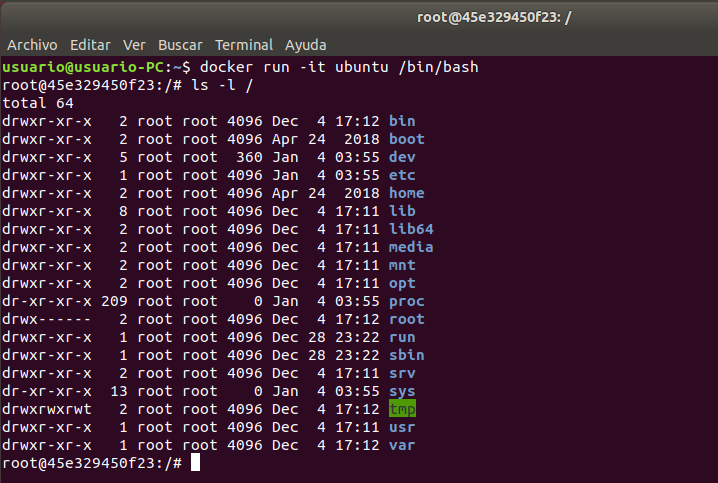
\includegraphics[width=\linewidth]{Trabajo/RecursosEducativos/RE05_Docker/Gestion_basica/REDocker_Gestion9.png}
	\vspace{-0.2cm}
	\caption{Salida comando docker run ubuntu ls -l /}
	\label{fig:DockerGestion9}
\end{figure}

Para poder salir de la terminal del contenedor se puede hacer de dos formas:
\begin{itemize}
    \item exit: El comando exit detiene la ejecución del contenedor y se regresará a la terminal del host.
    \item Ctrl+p+q: Al escribir la combinación de teclas se regresará a la terminal del host sin detener la ejecución del host.
\end{itemize}
%%%%%%%%%%%%%%%%%%%%%%%%%%%%%%%%%
%% INICIAR Y DETENER UN CONTENEDOR 
%%%%%%%%%%%%%%%%%%%%%%%%%%%%%%%%%
\textbf{Detener y reanudar contenedores}
Para detener la ejecución de un contenedor se utiliza el comando stop, pasando como argumento el identificador o el nombre del contenedor, de la siguiente forma

\begin{commandshell} docker stop 45e329450f23 \end{commandshell}

En caso de ser necesario, es posible detener todos los contenedores del host utilizando el comando stop de la siguiente forma

\begin{commandshell} docker stop \$(docker ps -a -q) \end{commandshell}

Para reanudar la ejecución de un contenedor que previamente ha terminado su ejecución se utiliza el comando start, pasando como argumento el identificador o el nombre del contenedor de la siguiente forma 

\begin{commandshell} docker start 45e329450f23 \end{commandshell}

\textbf{Conectarse a un contenedor}
Para conectarse a un contenedor que se encuentra en ejecución se utiliza el comando attach, pasando como argumento el identificador o nombre del contenedor de la siguiente forma

\begin{commandshell} docker attach 45e329450f23 \end{commandshell}

En la figura \ref{fig:DockerGestion10} se puede observar la conexión y ejecución del comando ls en un contenedor que se encontraba previamente en ejecución.

\begin{figure}[!hbtp]
	\centering
	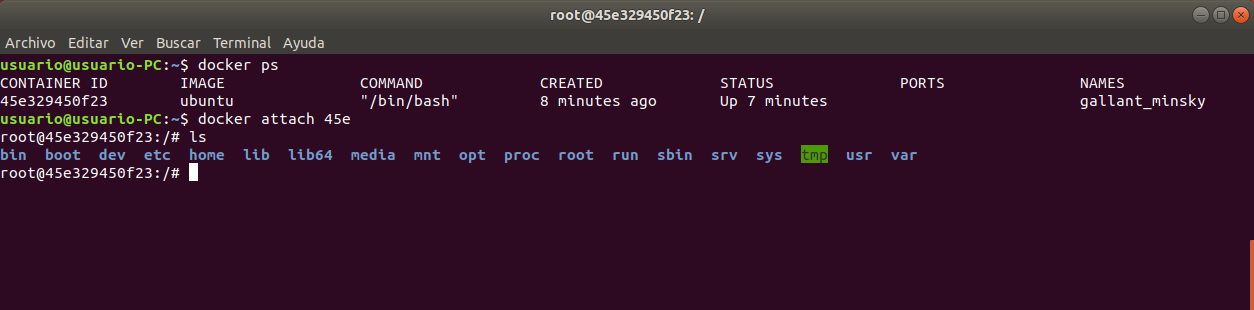
\includegraphics[width=\linewidth]{Trabajo/RecursosEducativos/RE05_Docker/Gestion_basica/REDocker_Gestion10.png}
	\vspace{-0.2cm}
	\caption{Conexión a contenedor en ejecución}
	\label{fig:DockerGestion10}
\end{figure}

%%%%%%%%%%%%%%%%%%%%%%%%%%%%%%%%%%%
%% ELIMINAR IMAGENES Y CONTENEDORES
%%%%%%%%%%%%%%%%%%%%%%%%%%%%%%%%%%%%
\textbf{Eliminar imágenes y contenedores}

Para eliminar un contenedor se requiere que este no se encuentre en ejecución, el comando rm se utiliza para eliminar un contenedor ingresando como argumento el identificador o el nombre del contenedor, de la siguiente forma
\begin{commandshell} docker rm 45e329450f23 \end{commandshell}

En caso de ser necesario, se pueden eliminar todos los contenedores del host utilizando el siguiente comando 
\begin{commandshell} docker rm $(docker ps -a -q)$ \end{commandshell}

Para eliminar una imagen que se encuentra descargada localmente se requiere que esta no tenga contenedores asociados. El comando para realizar la eliminación es rmi y recibe como argumento el identificador de la imagen a eliminar, de la siguiente forma

\begin{commandshell} docker rmi ubuntu \end{commandshell}

En caso de ser necesario, se pueden eliminar todas las imagenes del host utilizando el siguiente comando 
\begin{commandshell}docker rmi \$(docker images -q)\end{commandshell}

%%%%%%%%%%%%%%%%%%%%%%%%%%%%%%%%%%%
%% CONTENEDOR PERSONALIZADO 
%%%%%%%%%%%%%%%%%%%%%%%%%%%%%%%%%%%%
\textbf{Contenedor personalizado}
Para personalizar un contenedor se debe tener una conexión interactiva utilizando el siguiente comando
\begin{commandshell}docker run ubuntu /bin/bash \end{commandshell}

Una vez conectado al contenedor se procede a realizar las modificaciones necesarias, como la instalación de librerías, cambio de variables de entorno, gestión de archivos y directorios, un ejemplo sería la ejecución de los siguientes comandos
\begin{commandshellroot}
apt update
apt install net-tools
apt install nano
\end{commandshellroot}

%%%%%%%%%%%%%%%%%%%%%%%%%%%%%%%%%%%
%% IMAGEN PERSONALIZADA 
%%%%%%%%%%%%%%%%%%%%%%%%%%%%%%%%%%%%
\textbf{Imagen personalizada}
Para la creación de una imagen personalizada se utiliza el comando commit, el cual recibe como argumentos el identificador o nombre del contenedor y el nombre que va tener la imagen personalizada, como se puede ver en el siguiente comando

\begin{commandshell}docker commit 407b4c719d91 ubuntu-personalizado \end{commandshell}

En la figura \ref{fig:DockerGestion11} se puede observar la creación de una imagen personalizada y la verificación de que esta se encuentra disponible para su uso.

\begin{figure}[!hbtp]
	\centering
	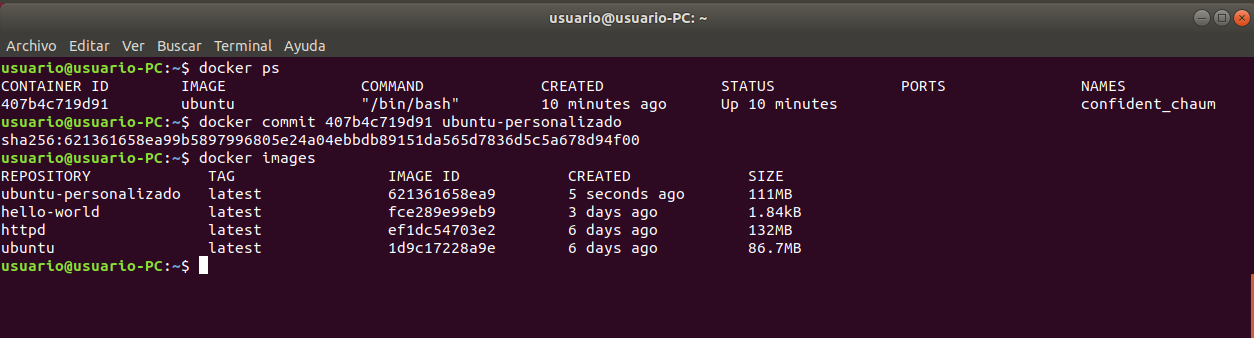
\includegraphics[width=\linewidth]{Trabajo/RecursosEducativos/RE05_Docker/Gestion_basica/REDocker_Gestion11.png}
	\vspace{-0.2cm}
	\caption{Creación imagen personalizada}
	\label{fig:DockerGestion11}
\end{figure}

\subsection{Caso resuelto}
El caso que se va realizar es la personalización de un contenedor y una imagen basada en ubuntu instalando el servidor Apache Web Server.

Para realizar la descarga de la imagen correspondiente se utiliza el comando

\begin{commandshell} docker pull ubuntu \end{commandshell}

Paso siguiente se crea un nuevo contenedor con el nombre de ubuntu-apache iniciando una consola interactiva, de la siguiente forma

\begin{commandshell} docker run --name ubuntu-apache -it ubuntu /bin/bash \end{commandshell}

Al estar en la terminal del contenedor se ejecutan los siguientes comandos para la instalación del servicio web de la siguiente forma 
\begin{commandshellroot}
apt update
apt install apache2
service start apache2
\end{commandshellroot}

Luego de instalados los paquetes necesarios e iniciado el servicio, se debe volver a la terminal del host y crear una imagen a partir del contenedor modificado previamente utilizando el siguiente comando

\begin{commandshell}
docker commit -c='CMD ["apache2ctl" , "-DFOREGROUND"]' \\
    -c 'EXPOSE 80' ubuntu-apache imagen-apache
\end{commandshell}

En el comando mostrado anteriormente, se realizan dos modificaciones importantes a la imagen: 
\begin{itemize}
    \item -c='CMD ["apache2ctl" , "-DFOREGROUND"]': Se agrega que al momento de su inicio se ejecute el servicio de apache en segundo plano.
    \item -c 'EXPOSE 80': Expone el puerto 80 de los contenedores creados con dicha imagen.
\end{itemize}

En la figura \ref{fig:DockerCaso1} se muestran la creación de la imagen personalizada a partir del contenedor ubuntu-apache.

\begin{figure}[!hbtp]
	\centering
	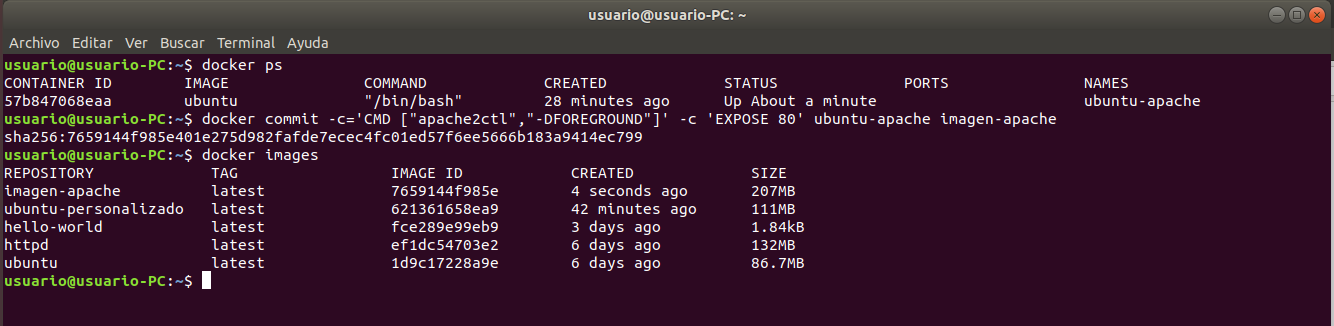
\includegraphics[width=\linewidth]{Trabajo/RecursosEducativos/RE05_Docker/Caso_resuelto/REDocker_Caso1.png}
	\vspace{-0.2cm}
	\caption{Creación imagen personalizada}
	\label{fig:DockerCaso1}
\end{figure}

Teniendo la imagen llamada imagen-apache disponible se procede a crear un nuevo contenedor basado en ella, utilizando el siguiente comando:

\begin{commandshell}
docker run --name nuevo-apache -d -p 8080:80 imagen-apache
\end{commandshell}

En el comando utilizado anteriormente resalta lo siguiente:
\begin{itemize}
    \item -d: Ejecuta el contenedor en segundo plano.
    \item -p 8080:80 : Permite que el puerto 80 del contenedor sea accedido a través del puerto 8080 del host.
    \item --name nuevo-apache: Nombre del contenedor.
\end{itemize}

En la figura \ref{fig:DockerCaso2} se muestra el proceso de creación y verificación del funcionamiento del contenedor llamado nuevo-ubuntu.

\begin{figure}[!hbtp]
	\centering
	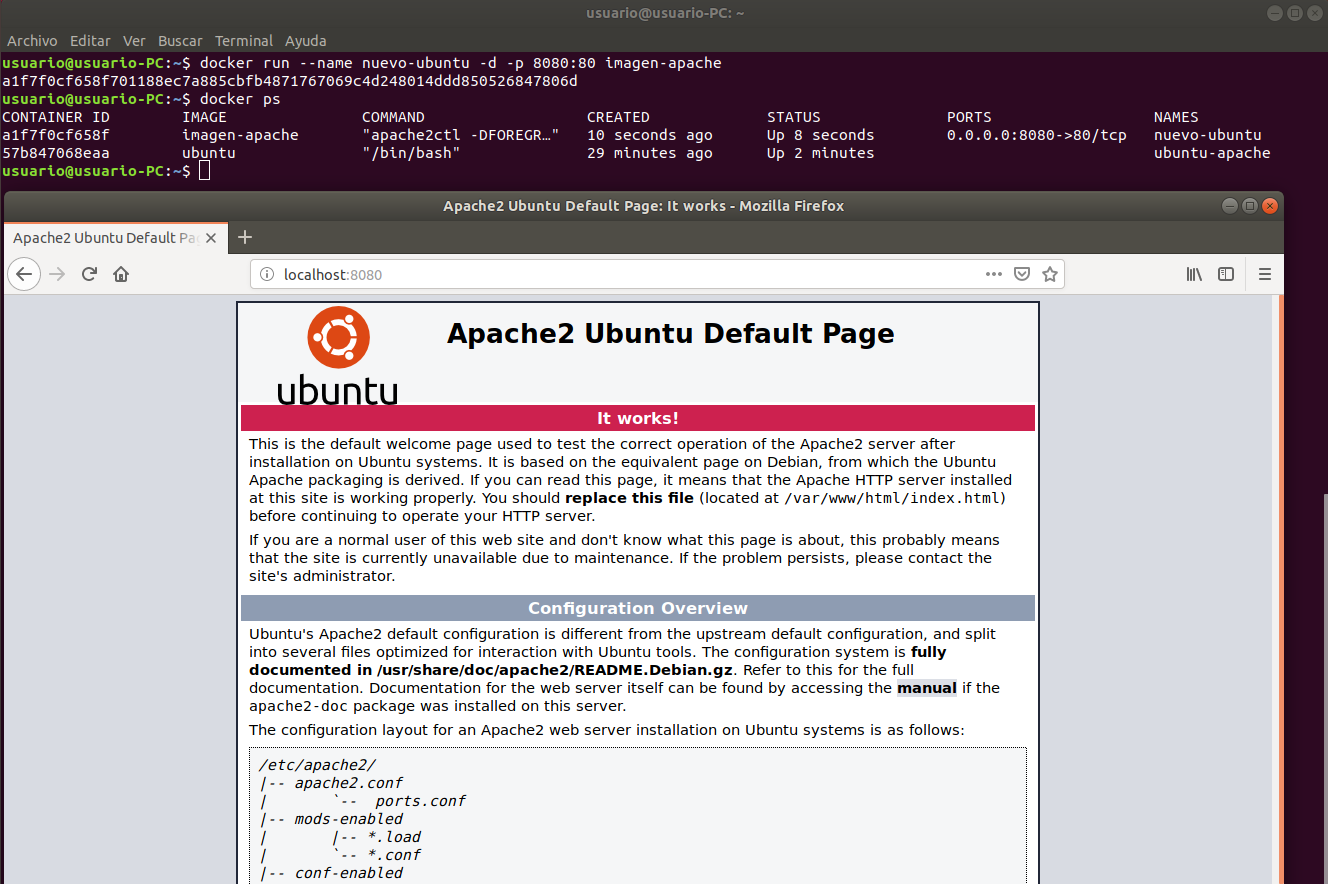
\includegraphics[width=\linewidth]{Trabajo/RecursosEducativos/RE05_Docker/Caso_resuelto/REDocker_Caso2.png}
	\vspace{-0.2cm}
	\caption{Creación imagen personalizada}
	\label{fig:DockerCaso2}
\end{figure}